\documentclass[t, xcolor={dvipsnames}]{beamer}

\usepackage{amsmath}
\usepackage{tipa}
\usepackage{eso-pic}
\usepackage{graphicx}
\usepackage{svg}
\usepackage{listings}
\usepackage{wrapfig}
\usepackage{scrextend}
\usepackage{subfig}
\usepackage[export]{adjustbox}

\setsvg{svgpath = img/}

\makeatletter
  \newenvironment{withoutheadline}{%
    \setbeamertemplate{headline}[default]
    \def\beamer@entrycode{\vspace*{-\headheight}}
    \setbeamertemplate{footline}[default]
  }{}
\makeatother

\usetheme{Malmoe}
\usecolortheme{dolphin}
\setbeamercolor{structure}{bg=red}

\title{\vspace{0.8cm}Automatic Birdsong Recognition}
\author{Victor F. L. Rodrigues}
\institute{School of Computer Science\\ The University of Manchester}
\titlegraphic{\includesvg[height=15mm]{UniOfManchesterLogo}}
\logo{\includesvg[height=10mm]{UniOfManchesterLogo}}

\begin{document}

%\usebackgroundtemplate{%
%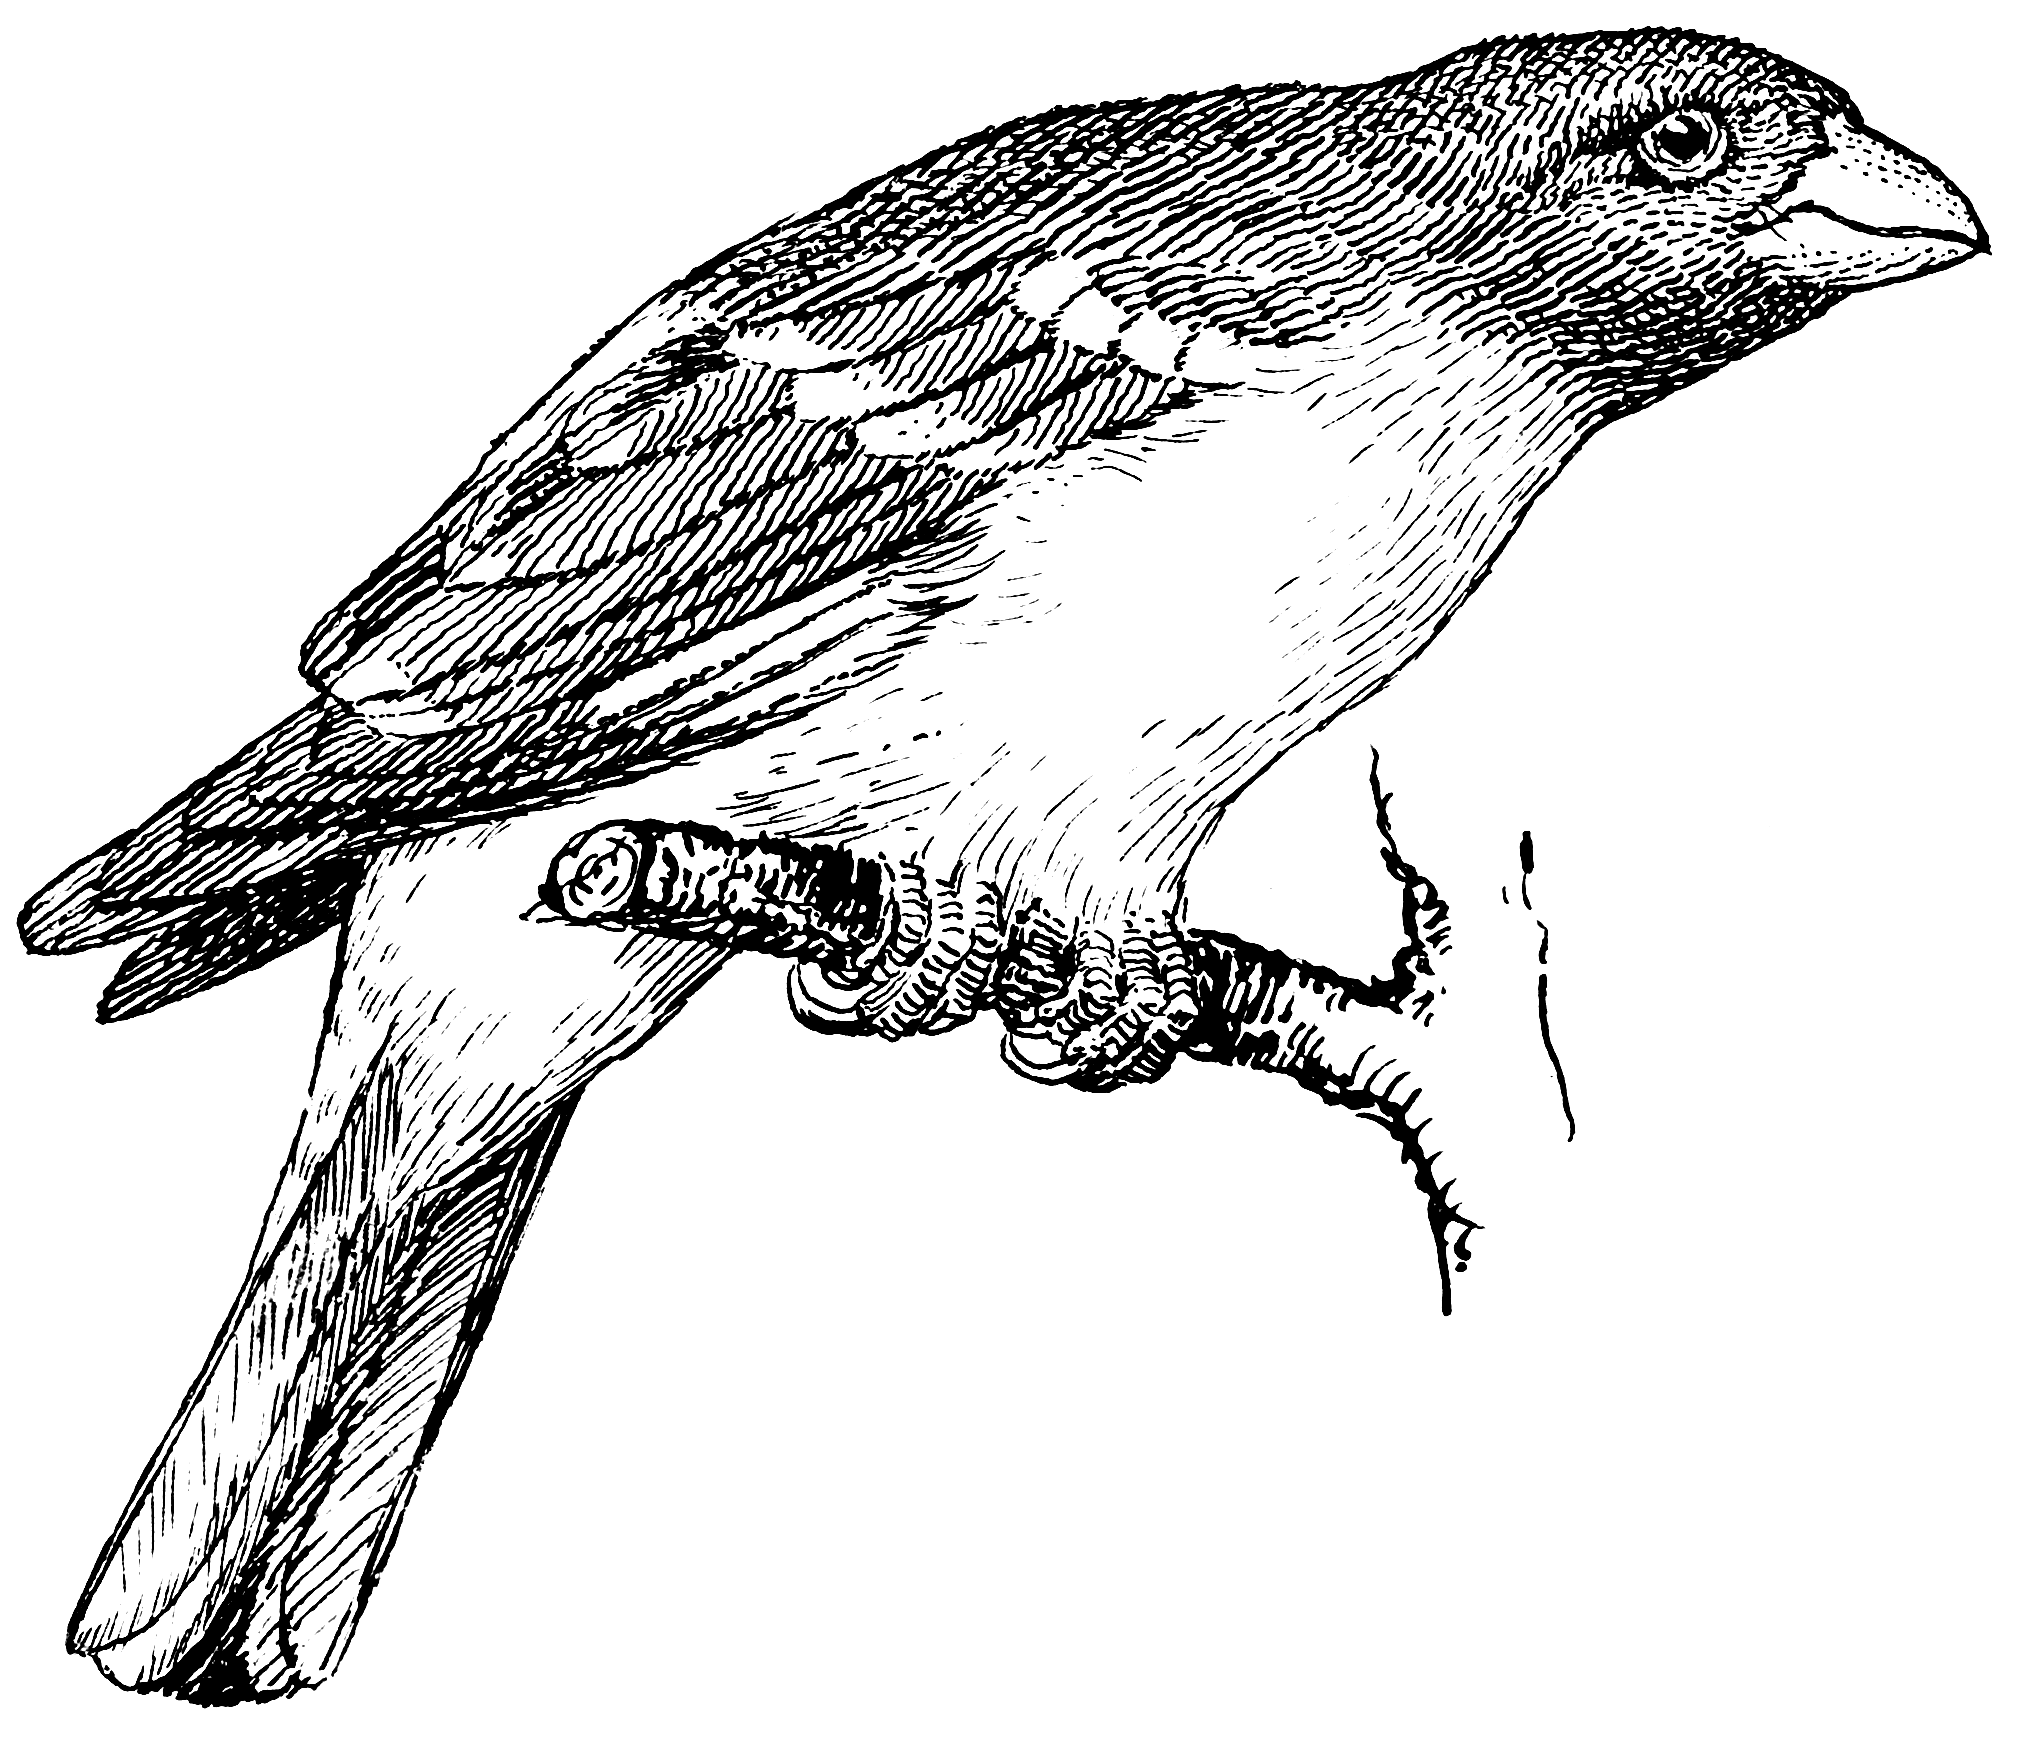
\includegraphics[width=0.5\paperwidth,height=0.5\paperheight,keepaspectratio=true]{img/Grossbeak_(PSF).png}
%}

\begin{withoutheadline}
  \begin{frame}[plain]
    \begin{wrapfigure}{L}[20cm]{0.23\textwidth}
      \vspace{0.2cm}
  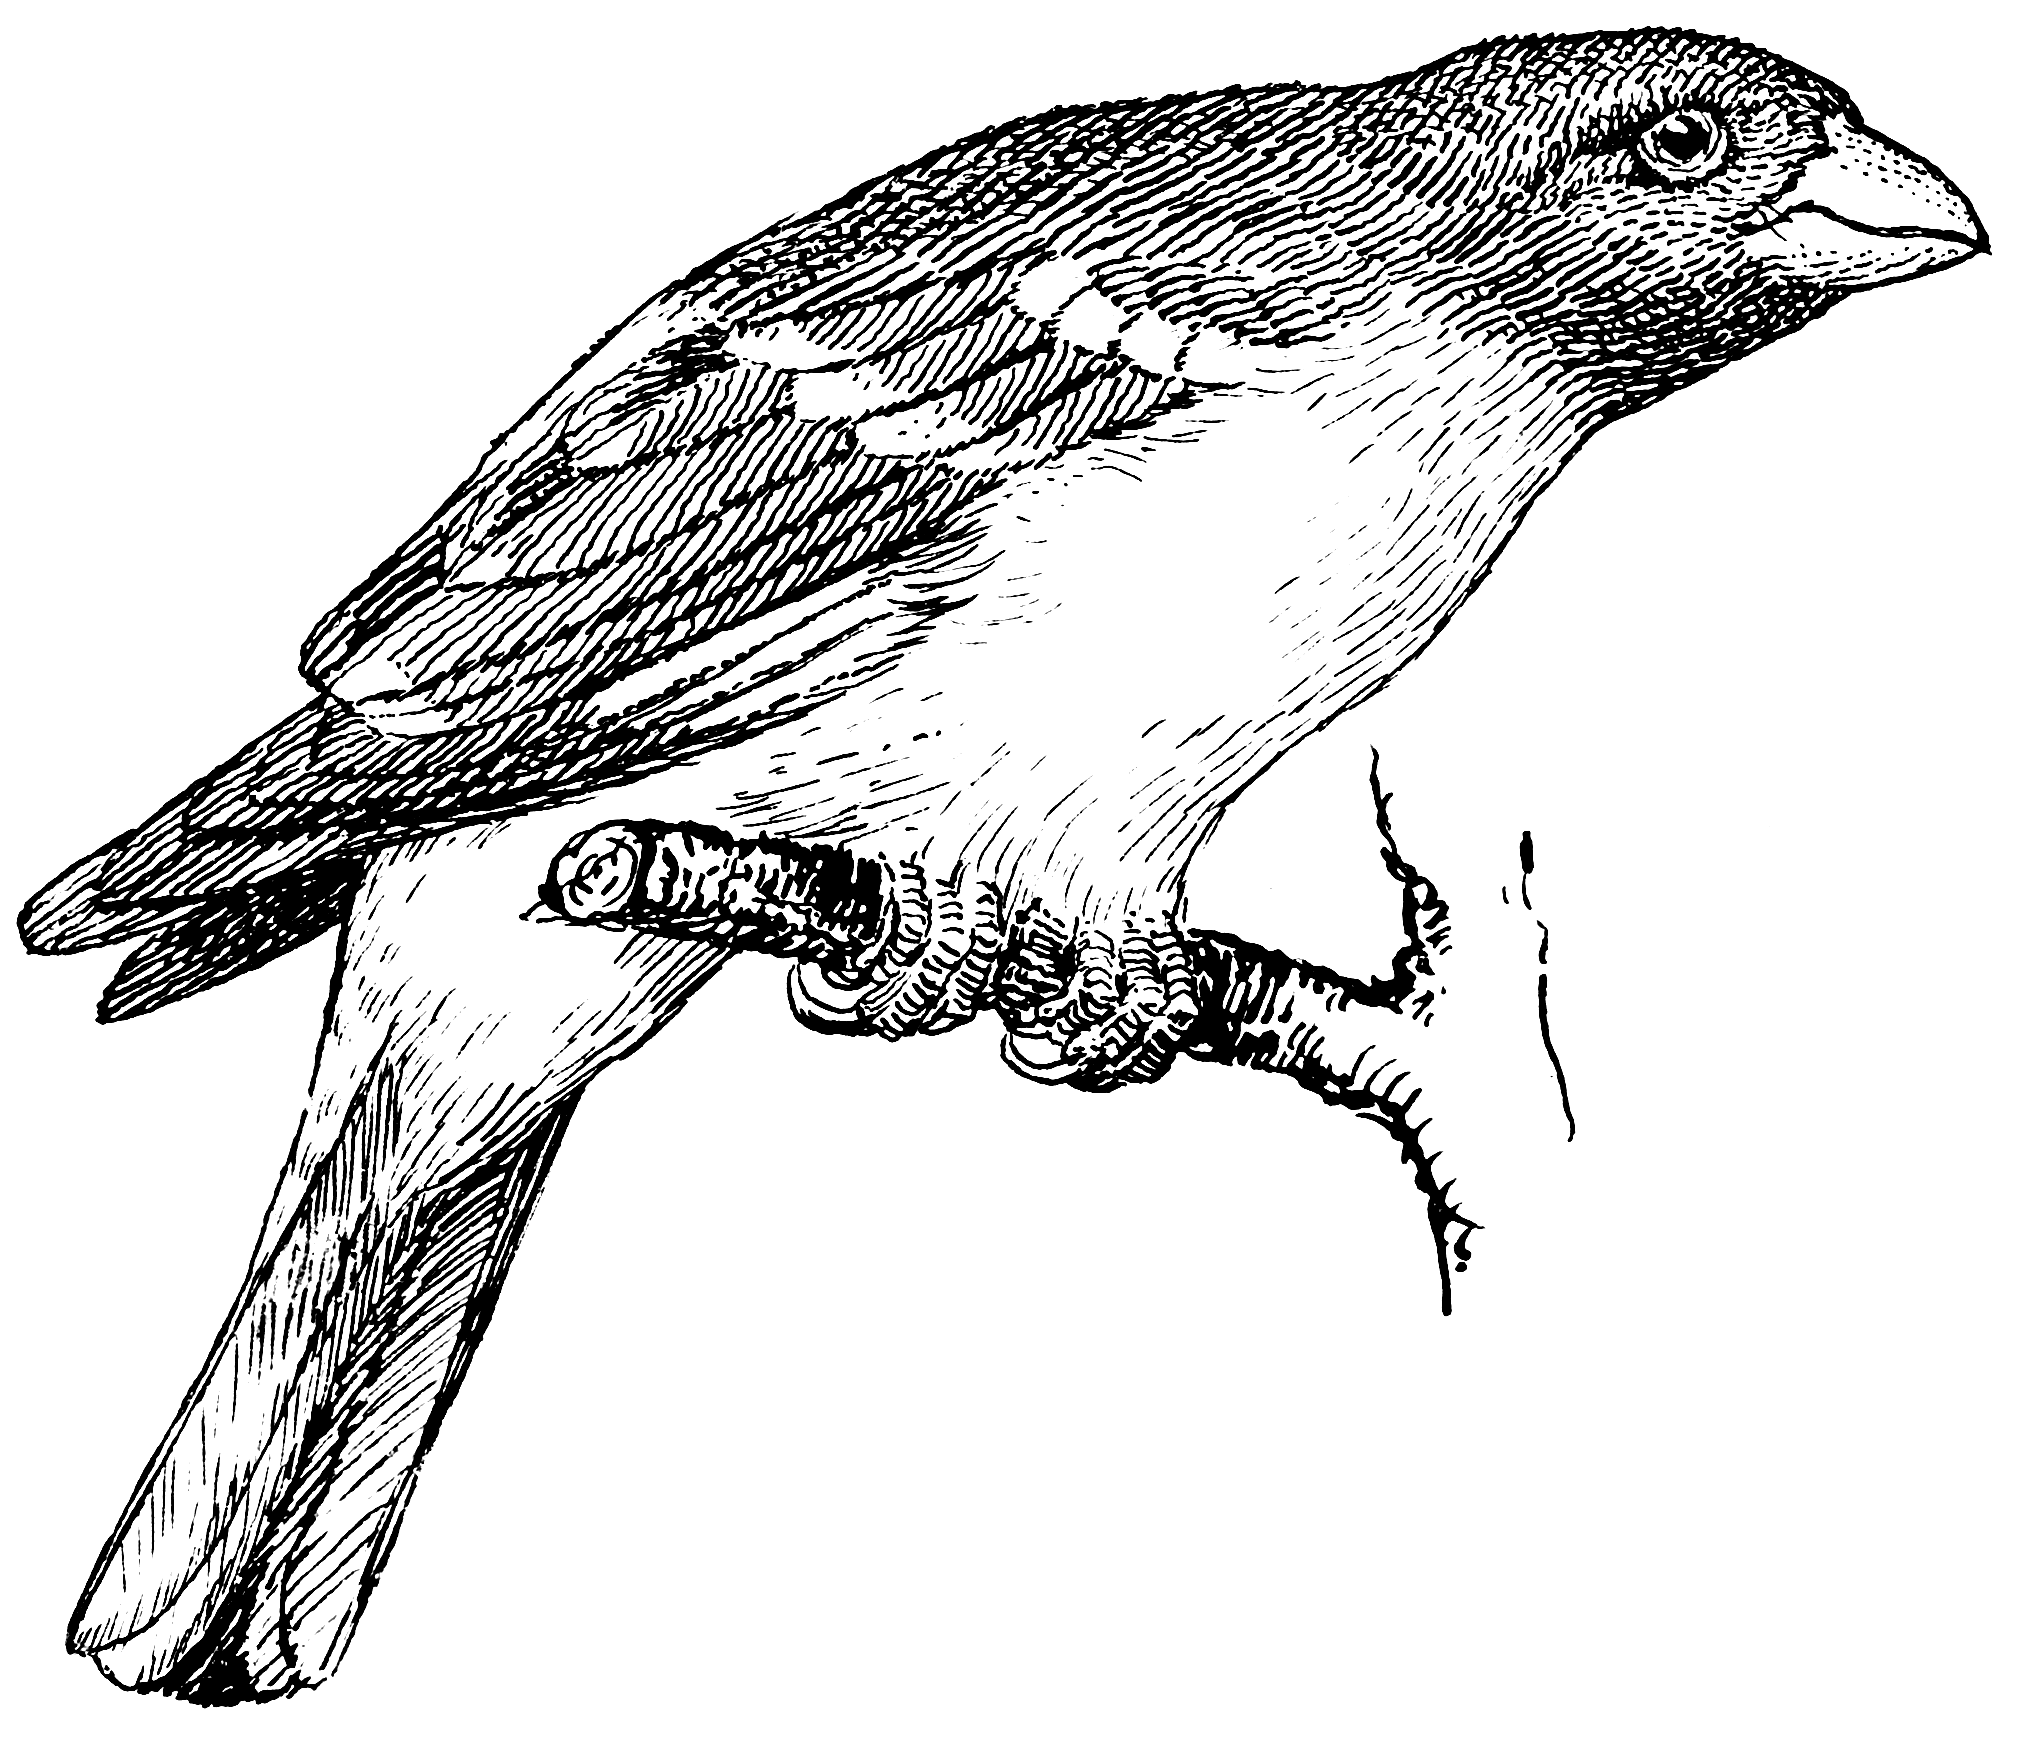
\includegraphics[width=0.5\paperwidth,height=0.5\paperheight,keepaspectratio=true]{img/Grossbeak_(PSF).png}
    \end{wrapfigure}
    \titlepage
  \end{frame}
\end{withoutheadline}

\usebackgroundtemplate{}

%-------------------------------------------------------------------------------

\section{Bird-Song Recognition}
\subsection{In Birdwatching}

\begin{frame}[fragile]
  \vspace{0.5cm}
  {\bfseries\Large How birdwatchers do it}\\
  \vspace{0.5cm}
  \begin{addmargin}{0.5cm}
    \begin{itemize}
      \item Listen for structure and composition:
      \begin{itemize}
        \item Linear tones
        \item Frequency sweeps
        \item Segment repetition
      \end{itemize}
      \item Through auditory perception or sonogram analysis
      \item May encounter difficulties:
      \begin{itemize}
        \item Multiple birds may be singing
        \item Some birds may mimic others
        \item Noisy environment
      \end{itemize}
    \end{itemize}
  \end{addmargin}
\end{frame}

%-------------------------------------------------------------------------------

\subsection{As a classification problem}

\begin{frame}[fragile]
  \vspace{0.5cm}
  {\bfseries\Large How a computer might do it}\\
  \vspace{0.5cm}
  \begin{addmargin}{0.5cm}
    \begin{itemize}
      \item This is a multi-class/multi-label classification problem
      \item Similar problems exist: Vocal recognition, music identification, whalesong classification\ldots
      \item Features are extracted from spectrographic analysis
      \item Machine learning is used to classify the data
      \item We must mitigate the same difficulties:
      \begin{itemize}
        \item Identify multiple, or ignore background species
        \item Distinguish similar birdsongs
        \item Apply noise reduction methods
      \end{itemize}
    \end{itemize}
  \end{addmargin}
\end{frame}

%-------------------------------------------------------------------------------

\section{Processing}

\begin{frame}[fragile]
  \vspace{0.5cm}
  {\bfseries\Large The data}
  \vspace{-0.15cm}
  \begin{figure}
    \includegraphics[clip, trim=0px 320px 0px 15mm, width=1.2\textwidth,center]{img/spec-wav}
  \end{figure}
\end{frame}

\begin{frame}[fragile]
  \vspace{0.5cm}
  {\bfseries\Large The data}
  \begin{figure}
    \includegraphics[clip, trim=0px 0px 0px 15mm, width=1.2\textwidth,center]{img/spec-wav}
  \end{figure}
\end{frame}

% In these frames talk about visible shapes and sweeps. maybe we could extract
% information or statistics on the frequency disitrbutions and the audiable
% repetitions? But maybe we have too much noise... leads to next section

%-------------------------------------------------------------------------------

\subsection{Noise Reduction}

\begin{frame}[fragile]
  \vspace{0.5cm}
  {\bfseries\Large Improving SNR}\\
  \vspace{0.5cm}
  \begin{addmargin}{0.5cm}
    \begin{itemize}
      \item Signal to noise ratio might interfere with feature extraction
      \item An \emph{automatic} noise reduction method is requried: \\
        less manual work means more data \& faster iteration
      \item Standard computer vision techniques can be used:
      \begin{itemize}
        \item Median filtering
        \item Thesholding
        \item Dilation \& Erosion\ldots
        \item Selective removal of small and/or generic components
      \end{itemize}
    % after a few parameter tweaks we get something more like this...  
    \end{itemize}
  \end{addmargin}
\end{frame}

% Too much noise to run edge detector. Some background noise is not part of the
% signal we are interested in. we want to minimise the SNR.
%
% Automatic noise reduction is necessary to increase the number of samples we
% can use. This is tricky, as noise reduction parameters are not global. We may
% need to automatically fit params to each recording, or make do with a general
% setting, which might be difficult to find.
%
% A combination of computer vision algos can be used
%
% We can apply median filtering for blurring purposes or as a method for
% thresholding, foe example, 1: 3*row,col, 0: otherwise. Blurring the image will
% effectively reduce the contrast of background noise, effectively smoothing it
% out allowing us to threshold it out.
%
% After blurring we can apply binary or limiting threshold to completely remove
% the noise.
%
% Once we have mostly only the important blocks we can dilate and erode in hopes
% of joining contiguous blocks and removing small segments completely.
%
% We can then remove any blocks smaller than a given amount as these usually
% don't belong to the signal we are focusing on, or are too generic to be of
% use.

%-------------------------------------------------------------------------------

\begin{frame}[fragile]
  \vspace{-0.5cm}
  \begin{figure}[!tfp]
    \centering
    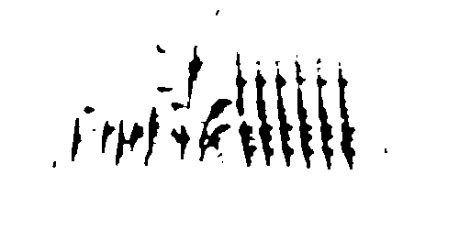
\includegraphics[width=0.8\textwidth]{img/specgram-long-clean}
  \end{figure}

  \vspace{-1cm}

  \begin{addmargin}{0.5cm}
    \begin{itemize}
      \item Global noise reduction parameters is won't work well for every recording
      \item But imperfect results might be close enough through statistical average
      \item Per-recording parameter fitting would be ideal, but more complex
    \end{itemize}
  \end{addmargin}
\end{frame}

% Point out imperfect cleanup. Note that this is impossible w/ global
% parameters, but maybe it doesn't have to be perfect in the first place given
% the quantity of samples that we will have.

%-------------------------------------------------------------------------------

\subsection{Feature Engineering}
\begin{frame}[fragile]
  \vspace{0.5cm}
  {\bfseries\Large Retrieving information}\\
  \begin{figure}
    \includegraphics[clip, trim=0px 1cm 0px 350px, width=1.2\textwidth,center]{img/spec-wav}
  \end{figure}
  \vspace{-0.3cm}
  \begin{addmargin}{0.5cm}
    \begin{itemize}
      \item Dominant frequency domains (pitch)
      \item Characteristic sweeps and tones
      \item Structure:
      \begin{itemize}
        \item repeating components (syllables)
        \item repeating segments
        \item repeating songs
      \end{itemize}
    \end{itemize}
  \end{addmargin}
\end{frame}

%-------------------------------------------------------------------------------

\begin{frame}[fragile]
  \vspace{0.5cm}
  \begin{addmargin}{0.5cm}
    \begin{itemize}
      \item Image recognition can be used\ldots
      \item Components or segments can be cross-correlated against spectrograms
      \item A common approach is template matching:
    \end{itemize}
  \end{addmargin}

    \begin{figure}[!tbp]
      \centering
      \begin{minipage}[c]{0.3\textwidth}
        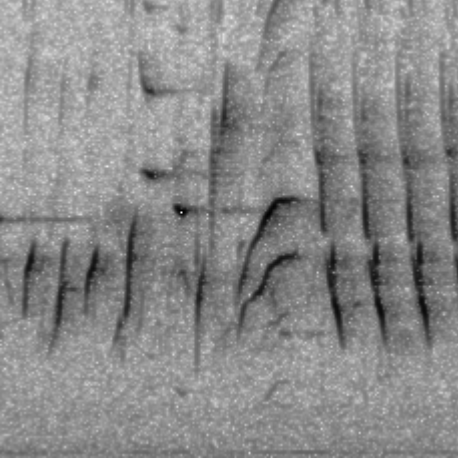
\includegraphics[width=\textwidth]{img/specgram}
      \end{minipage}
      \hfill
      \begin{minipage}[c]{0.3\textwidth}
        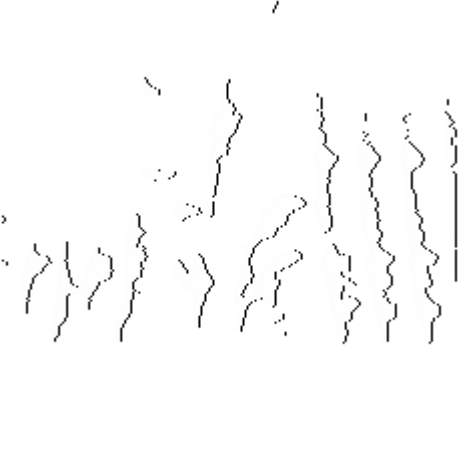
\includegraphics[width=\textwidth]{img/contours}
      \end{minipage}
      \hfill
      \begin{minipage}[c]{0.3\textwidth}
        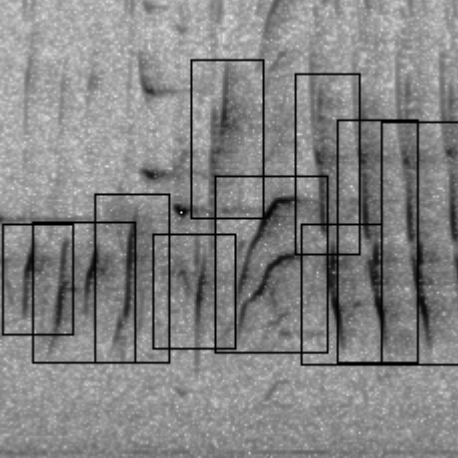
\includegraphics[width=\textwidth]{img/detected-features}
      \end{minipage}
    \end{figure}
\end{frame}

\begin{frame}[fragile]
  \vspace{0.5cm}
  \begin{addmargin}{0.5cm}
    \begin{itemize}
      \item Image recognition can be used\ldots
      \item Components or segments can be cross-correlated against spectrograms
      \item A common approach is template matching:
    \end{itemize}

  \end{addmargin}
    \begin{figure}[!tbp]
      \centering
      \begin{minipage}[c]{0.3\textwidth}
        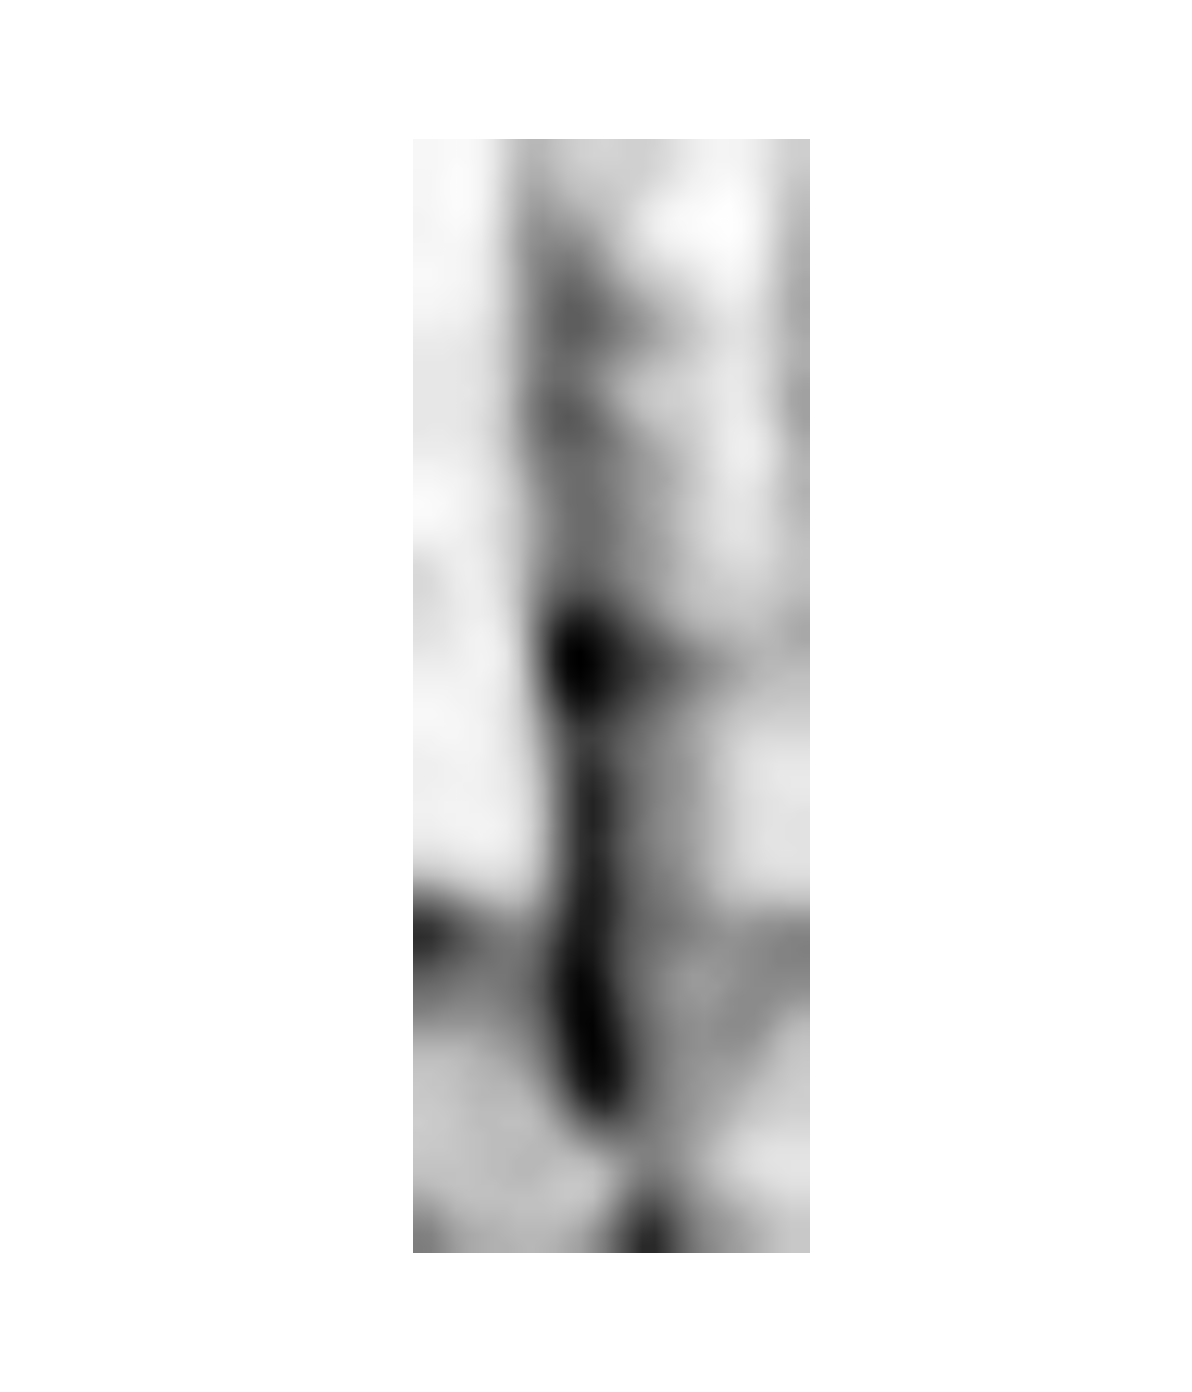
\includegraphics[width=\textwidth]{img/selected-feature}
      \end{minipage}
      \hfill
      \begin{minipage}[c]{0.3\textwidth}
        \fbox{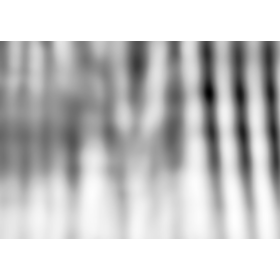
\includegraphics[width=\textwidth]{img/ccm}}
      \end{minipage}
      \hfill
      \begin{minipage}[c]{0.3\textwidth}
        \fbox{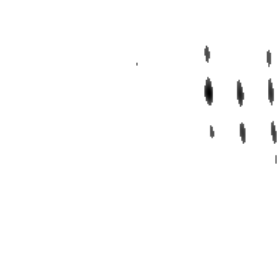
\includegraphics[width=\textwidth]{img/threshold-ccm}}
      \end{minipage}
    \end{figure}
\end{frame}


%-------------------------------------------------------------------------------

\section{Classification}
\subsection{Training}
\begin{frame}[fragile]
  \vspace{0.5cm}
  {\bfseries\Large Classifier training}\\
  \vspace{0.5cm}
  \begin{addmargin}{0.5cm}
    \begin{itemize}
      \item Cross-correlation maps are used as similarity vectors
      \item Component and segment detection provides composition statistics, as well as frequency distribution for each species
      \item Many classifiers can be used, but we'll use decision trees (for now)
      \item Multiple, in fact: A random forest of 50--500 trees\ldots per class
    \end{itemize}
  \end{addmargin}
\end{frame}

\subsection{Classification}
\begin{frame}[fragile]
  \vspace{0.5cm}
  {\bfseries\Large Classification}
  \vspace{0.5cm}
  \begin{addmargin}{0.5cm}
    \begin{itemize}
      \item Template matching is performed, producing a similarity feature vector
      \item Noise reduction is applied and component detection is performed on the target spectrogram, producing statistics
      \item These are fed into each RF, and the maximal probability is accepted
    \end{itemize}
  \end{addmargin}
\end{frame}

\subsection{Accuracy and Performance}
\begin{frame}[fragile]
  \vspace{0.5cm}
  {\bfseries\Large Classifying accuracy}
  \vspace{0.5cm}
  \begin{addmargin}{0.5cm}
    \begin{itemize}
      \item Receiver Operating Characteristic (ROC) is compiled from true-positive and false-positive rates
      \item Accuracy is determined by the area under the ROC curve (AUC) per classifier
      \item The goal is to maximize this area
      \item Overall accuracy computed by averaging all classifier AUC results
    \end{itemize}
  \end{addmargin}
\end{frame}

\begin{frame}[fragile]
  \vspace{0.5cm}
  {\bfseries\Large Improving performance}
  \vspace{0.5cm}
  \begin{addmargin}{0.5cm}
    \begin{itemize}
      \item High feature count and template matching contribute to high computational costs
      \item Discarding less important features should improve accuracy and performance
      \item Template matching can be sped up by blurring templates and target image
      \item We should exploit parallelization and optimizations provided by existing libraries
    \end{itemize}
  \end{addmargin}
\end{frame}


%-------------------------------------------------------------------------------

\section{}
\begin{frame}[fragile]
  general diagram showing entire workflow from preprocessing to accuracy classification
\end{frame}

\begin{frame}[fragile]
  \vspace{0.5cm}
  {\bfseries\Large Summary}\\
  \vspace{0.3cm}
  %\begin{addmargin}{0.5cm}
    \begin{itemize}
      \item Automatic birdsong recognition features similar problems to manual classification
      \item Manual pre-processing is slow, automatic methods are necessary
      \item Birdsong can be simple or complex. data must be engineered to extract meaningful information across all species
      \item Classifier accuracy feedback will allow us to tune parameters
      \item Immense amounts of data and CV processing can pose computational issues
    \end{itemize}
  %\end{addmargin}
\end{frame}

\begin{frame}[fragile]
  \vspace{0.5cm}
  \begin{addmargin}{0.5cm}
    Attributions/bib...
  \end{addmargin}
\end{frame}


%-------------------------------------------------------------------------------

% \begin{frame}[fragile] \vspace{0.5cm} {\bfseries\Large title}\\ \vspace{0.5cm}
% \begin{addmargin}{0.5cm} ASDASFASFASFASFSF \begin{itemize} \item problem
% statement \item traditional methods \item this is a multi-class, maybe
% multi-label classification problem \item what does the data look like (show
% specgram, don't explain too much) \item view as a spectrogram \item modern
% approaches \end{itemize} \end{addmargin} \end{frame}
% 
% %-------------------------------------------------------------------------------
% 
% \begin{frame}[fragile]
%   \vspace{0.5cm}
%   {\bfseries\Large title}\\
%   \vspace{0.5cm}
%   \begin{addmargin}{0.5cm}
%     \begin{itemize}
%       \item back to spectrogram, show energy, show structure. show plain PCM and compare information richness
%       \item maybe show examples of messy specgrams
%       \item noise reduction
%       \item can use simple methods, median filtering dilation etc
%       \item doesn't have to be perfect
%       \item must be AUTOMATIC, more samples -> more data
%     \end{itemize}
%   \end{addmargin}
% \end{frame}
% 
% %-------------------------------------------------------------------------------
% 
% \begin{frame}[fragile]
%   \vspace{0.5cm}
%   {\bfseries\Large title}\\
%   \vspace{0.5cm}
%   \begin{addmargin}{0.5cm}
%     \begin{itemize}
%       \item now w/ clear audio, feature extraction
%       \item look at structure, speculate on interesting features
%       \item retrieve statistics -- distribution across freqs...
%       \item contiguous blobs, contours, bounding box
%       \item extract from unprocessed specgram, gauss blur, use as feature
%       \item explain correlation map, use of tmplate matching with target specgram
%       \item show threshold of this to demonstrate multiple matches
%     \end{itemize}
%   \end{addmargin}
% \end{frame}
% 
% %-------------------------------------------------------------------------------
% 
% \begin{frame}[fragile]
%   \vspace{0.5cm}
%   {\bfseries\Large title}\\
%   \vspace{0.5cm}
%   \begin{addmargin}{0.5cm}
%     \begin{itemize}
%       \item classification
%       \item lots of parameters, speculate automatic fitness of cleanup, feature extraction
%       \item train tree
%       \item train lots of trees, 50 or 500 -- random forest
%       \item 1 forest per class (species)
%       \item classifier training will determine best splits
%       \item features that are used: template matching, ...
%       \item for template matching we can reduce resolution and downsample to improve performance
%     \end{itemize}
%   \end{addmargin}
% \end{frame}

\end{document}
